\documentclass[a4paper]{llncs}
\usepackage[T1]{fontenc}
\usepackage[hyphens]{url}
\usepackage{graphicx}
\urlstyle{rm}
\def\UrlFont{\rm}
\usepackage{amsmath}
\usepackage{amssymb}
\usepackage{booktabs}
\usepackage{array}
\usepackage{multirow}
\usepackage{algorithm}
\usepackage{algorithmic}
\usepackage{microtype}

\newcommand{\cmark}{$\checkmark$}
\newcommand{\xmark}{$\times$}
\newcommand{\subfigtext}[1]{\par\vspace{0.25em}\centering\small #1\par}

\title{ShapeShift: Active-Shape Scheduling for Diffusion Language Model Serving}
\titlerunning{ShapeShift: Active-Shape Scheduling for dLLM Serving}
\author{Kexin Chu}
\authorrunning{K. Chu}
\institute{University of Connecticut\\ \email{kexin.chu@uconn.edu}}

\begin{document}
\maketitle

\begin{abstract}
Diffusion language models (dLLMs) generate by repeatedly updating a prompt-response canvas rather than extending a cached prefix one token at a time. This execution model creates a serving bottleneck that is easy to miss in single-request inference: when short and long requests share a denoising step, the transformer body runs at the longest sequence shape, so shorter requests repeatedly pay padding work created by their batch companions. We identify this effect as \emph{long-context shape waste} and show that it is an online scheduling problem. We present \emph{ShapeShift}, an active-shape continuous batching runtime that treats sequence length as a step-level scheduling resource. ShapeShift chooses an anchor request, fills the step batch with nearest-length companions, filters additions that would create excessive rectangular work, and uses service-gap aging to keep old or shape-outlier requests in service. Integrated into dlmserve, ShapeShift improves online throughput by 1.11--2.15$\times$ over FCFS across four open checkpoints and mixed-length serving traces, while reducing mean and p95 request latency. Against stronger length-aware baselines on LLaDA-8B, it achieves the best throughput--tail trade-off on heterogeneous queues (2.15$\times$ throughput at 0.54$\times$ p95 latency on OpenOrca). Longer-horizon validation across five workloads shows 1.14--1.88$\times$ throughput gains. The gains concentrate in the predicted regime: backlogged, shape-heterogeneous ready pools where active step-batch selection can prevent repeated long-shape co-residence.
\end{abstract}
\keywords{Diffusion language models \and Serving systems \and Resource management and scheduling \and Parallel inference}

\section{Introduction}

Autoregressive (AR) LLMs power most production text services, but token-by-token decoding keeps generation sequential. Diffusion language models (dLLMs) instead allocate a response canvas, mask unknown positions, and repeatedly denoise the full prompt-response canvas with a bidirectional transformer. Recent dLLM checkpoints and serving systems~\cite{ssdlm2022,diffullama2024,nie2025llada,dream2025,coda2025,llada20_2025,illada2026,zhao2025fastdllm,dInfer2025,dllmserve2025} make this family increasingly practical. Shared serving exposes a batching problem absent in single-request inference: each denoising step revisits the full canvas, so a short request batched with a long one can repeatedly inherit the long request's sequence shape.

AR serving systems optimize prefill/decode disaggregation, speculation, multi-tenant batching, and KV reuse~\cite{splitwise2023,specinfer2024,medusa2024,eagle2024,tetriinfer2024,punica2023,slora2023,muxserve2024,loongserve2024,alignedserve2026,laps2026,mcam2025}. Recent dLLM systems reduce the cost of a chosen denoising step~\cite{zhao2025fastdllm,dInfer2025,dllmserve2025}, but the serving loop still decides which active requests create the update shape. An online dLLM server can therefore waste transformer-body work by repeatedly co-scheduling long and short canvases in the same step batch.

Our key observation is that this waste is a scheduling effect. In GPU probes across three dLLM checkpoints, mixed short/long batches take essentially the same time as all-long batches over the same denoising steps. Once a long request enters a step batch, every shorter companion is charged for the long rectangular shape at each co-scheduled step. We call this effect \emph{long-context shape waste}. It changes the runtime interpretation of sequence length: length is not only an admission-time property, but a repeated-step resource that should be controlled whenever the active set is rebatched.

This view shifts the serving question from ``how fast can the next update run?'' to ``which active sequence shapes should run together?'' The distinction matters because an update can be locally optimized by kernels or caches while still being globally inefficient for the ready pool if its batch shape is dominated by a long outlier. ShapeShift targets this missing active-set decision.

We design \emph{ShapeShift}, an active-shape scheduler for dLLM continuous batching. ShapeShift makes one local decision at each scheduler tick: which ready requests should share the next denoising step. It chooses an anchor request to define the length region of the step, fills with nearest-length companions to reduce rectangular padding, filters candidates that would create excessive padded work, and promotes overdue requests through service-gap aging. These rules are deliberately step-level rather than admission-level: a request may need different companions as other requests arrive, finish, or become overdue.

We integrate ShapeShift into dlmserve and evaluate it with direct online arrivals from serving-oriented workloads, including ShareGPT long-context chat, Wikipedia-style multi-hop QA, instruction mixes, and heterogeneous multi-task queues. The evaluation follows the mechanism: cross-model runs measure end-to-end serving gains, ablations separate active-shape batching from compactness and aging controls, length-aware baselines test whether step-level selection adds value beyond coarse grouping, and boundary sweeps identify when the ready pool contains enough backlog and length diversity for shape-compatible batching.

This paper makes the following contributions.

\begin{enumerate}
  \item We identify \emph{long-context shape waste}: in dLLM serving, short requests can repeatedly pay the transformer-body cost of the longest request in their denoising step batch.
  \item We design and implement \emph{ShapeShift}, a step-level scheduler that combines anchor-based nearest-length batching, compactness filtering, and service-gap aging to control padding while preserving regular service for unusual-length requests.
  \item We evaluate ShapeShift on online dLLM serving workloads across four open checkpoints and five scheduler policies, showing up to 2.15$\times$ throughput improvement over FCFS with lower mean and p95 latency, and characterize the backlog and heterogeneity regimes where active-shape scheduling is most effective.
\end{enumerate}

\section{Background and Motivation}

\subsection{Step Batches and Rectangular Shape}

Let a request have prompt length $P$, generation canvas length $G$, and total sequence length $L=P+G$. Prompt-invariance certificates~\cite{zhang2026pi} constrain prompt content; they leave the length term $P$ inside the rectangle. A dLLM denoising step runs the transformer over the current prompt-response canvas, whose unknown output positions are represented by mask tokens. For serving, the important property is that each step processes the whole canvas rather than appending one token to a cached prefix.

When a server batches multiple active requests at a denoising step, the requests must share a common sequence dimension. A step batch $\mathcal{B}$ is therefore padded to its longest member and executes as a rectangle with token-row size
\[
  |\mathcal{B}|\cdot L_{\max}(\mathcal{B}), \quad
  L_{\max}(\mathcal{B})=\max_{r\in\mathcal{B}} L_r .
\]
Only $\sum_{r\in\mathcal{B}} L_r$ token rows correspond to actual request content. We use the shape-padding ratio
\[
  \rho(\mathcal{B}) =
  \frac{|\mathcal{B}|\cdot L_{\max}(\mathcal{B})}
       {\sum_{r\in\mathcal{B}} L_r}
\]
as a scheduler-facing proxy for avoidable rectangular work. The metric captures the part of step cost that changes when the scheduler changes which canvases co-reside; all experiments keep model kernels and generation settings fixed across schedulers.

\subsection{Why Shape Matters Repeatedly}

Length-aware scheduling already appears in AR serving, but dLLMs amplify the consequence of poor length pairing. In AR serving, a long prompt mainly increases prefill cost; later decode iterations reuse a KV cache and add one token per request. In a dLLM, the same prompt-response canvas is revisited over many denoising steps. If a 2K-token request is repeatedly batched with much shorter requests, those shorter requests repeatedly execute under the 2K-token rectangular shape.

This repeated shape effect separates model-side dLLM acceleration from serving-side scheduling. Cache reuse, sparse attention, and parallel decoding reduce the cost of a chosen step, while active-shape scheduling decides which ready requests create that step shape. FCFS is a natural online baseline because it preserves arrival order, but its ordering rule is unrelated to shape compatibility. The scheduler therefore needs a second notion of locality beyond arrival time: which active canvases should co-reside in the next rectangular step.

\begin{figure}[t]
  \centering
  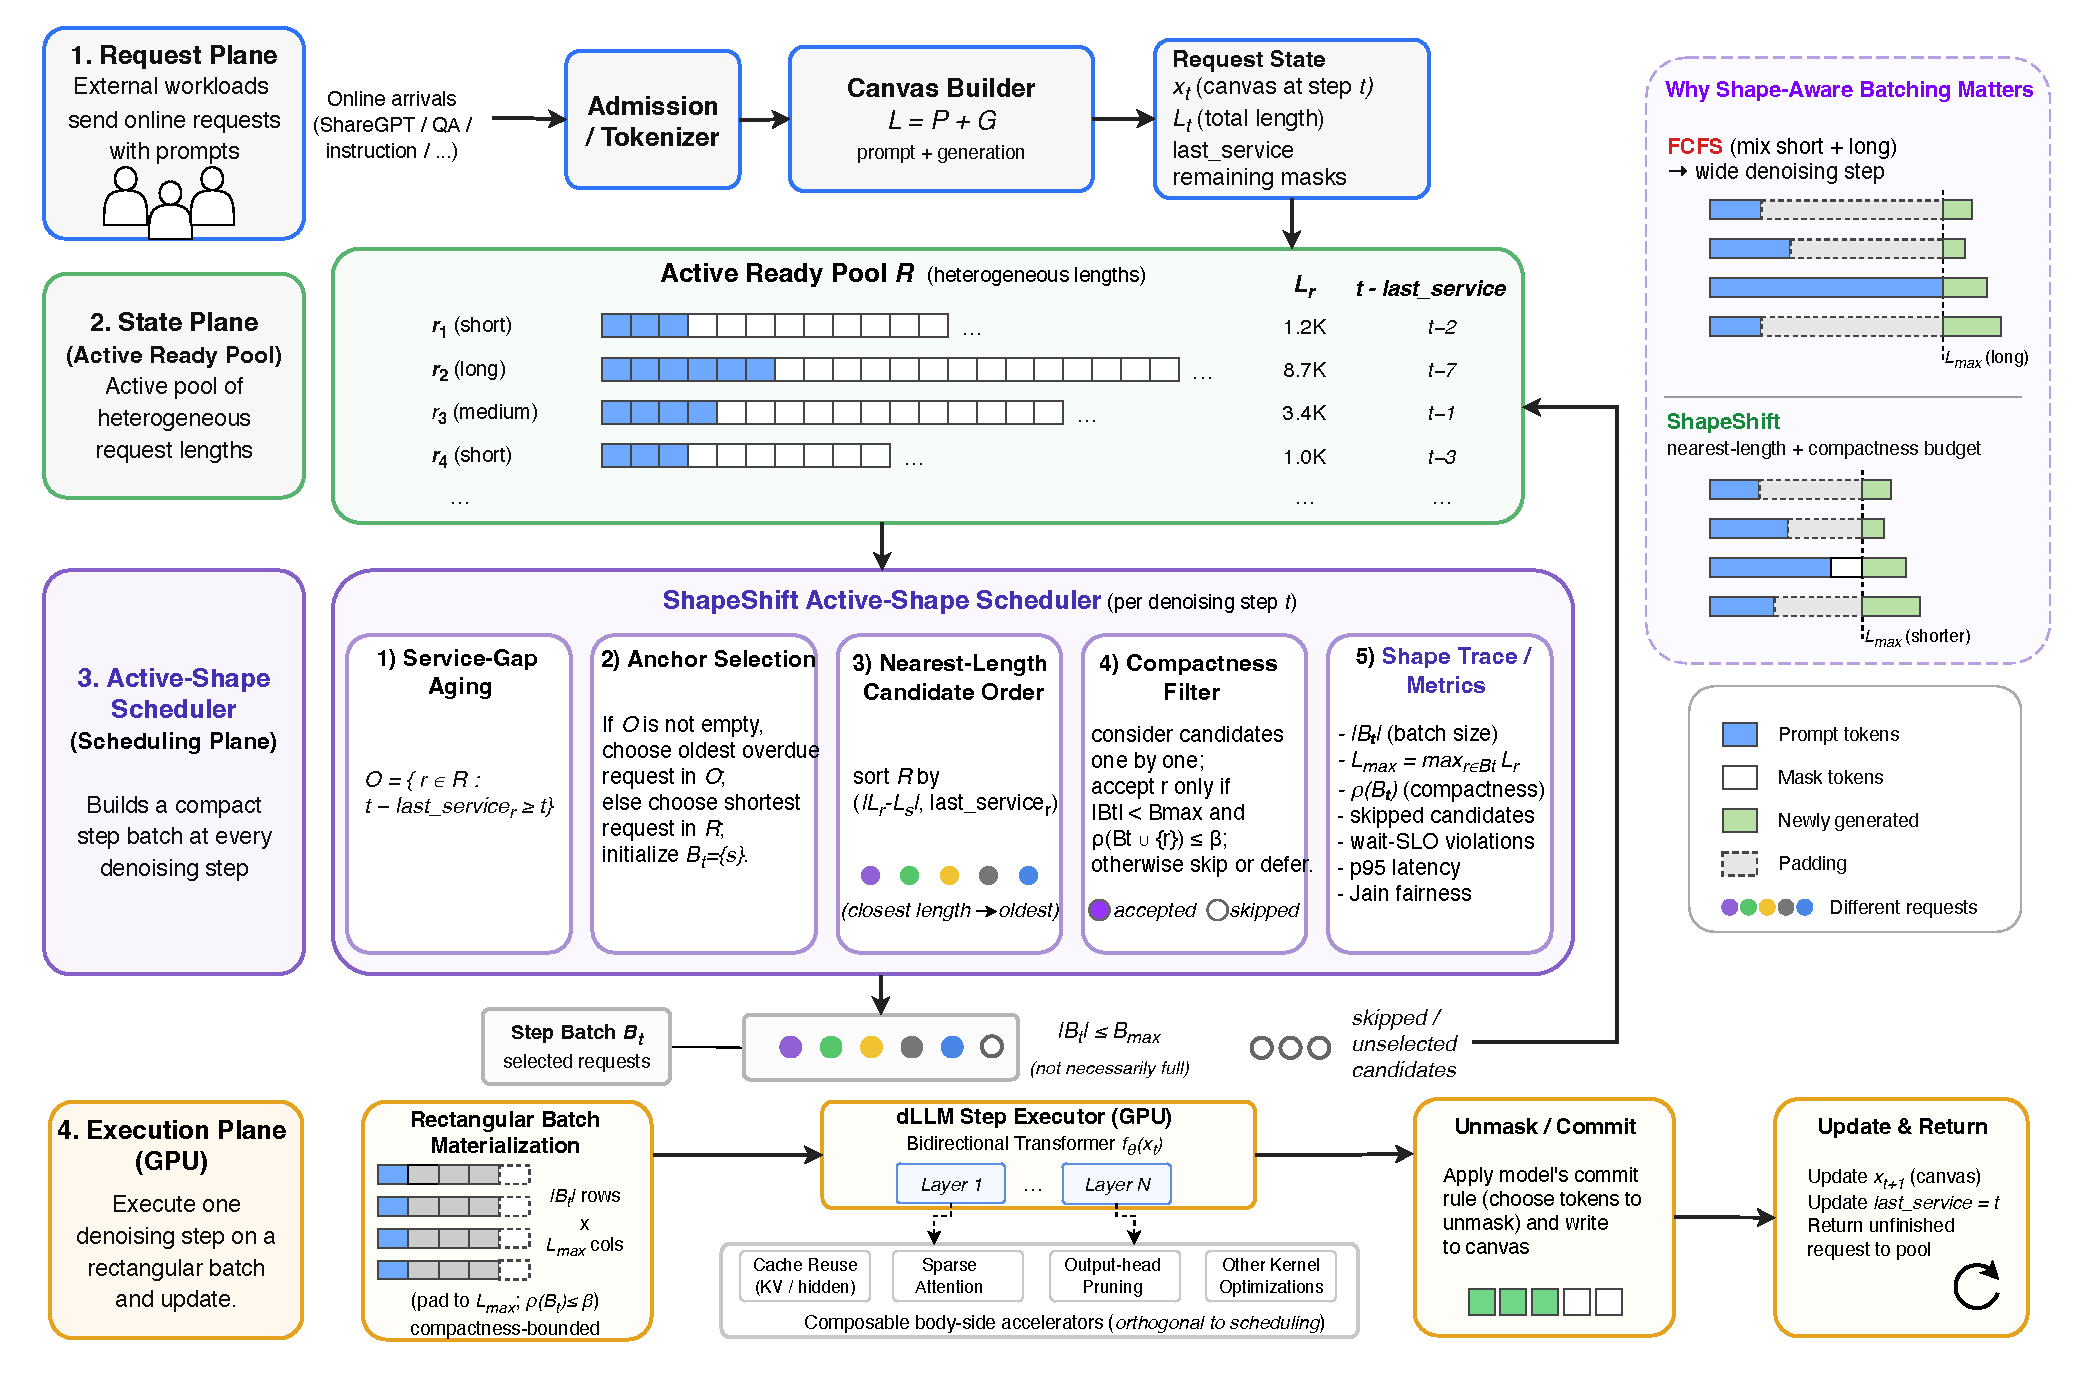
\includegraphics[width=0.9\linewidth]{figures/ShapeShift-Arch.pdf}
  \caption{ShapeShift serving loop and active-shape scheduler for step-level dLLM batching.}
  \label{fig:design-overview}
\end{figure}

\subsection{Motivating Observations}

\textbf{Observation 1: online dLLM traces are shape-heterogeneous.} We build length traces from ShareGPT using the LLaDA tokenizer. Single-turn requests are mostly short but have a long tail, while multi-turn accumulated requests often approach the serving-window limit. This spread creates a scheduling opportunity: FCFS can repeatedly pull short requests up to tail shapes, while shape-aware scheduling can group compatible canvases.

\textbf{Observation 2: mixed-length batches behave like long batches.} We run a controlled GPU microbenchmark on three dLLM checkpoints with a 128-token output canvas, 128 denoising steps, batch size four, and total canvas lengths of 256 (short) and 2048 (long). Table~\ref{tab:motivation-probe} reports end-to-end latency for all-short, all-long, and mixed (two short, two long) batches. Across checkpoints, the mixed batch is nearly as expensive as the all-long batch.

\begin{table}[t]
\centering
\caption{Controlled GPU microbenchmark: latency for all-short (256 tokens), all-long (2048 tokens), and mixed batches (two short, two long) with a shared 128-token output canvas and 128 denoising steps. ``Mix/long'' is mixed latency divided by all-long latency.}
\label{tab:motivation-probe}
\scriptsize
\setlength{\tabcolsep}{2.8pt}
\begin{tabular}{lcccc}
\toprule
Model & All short & All long & Mixed & Mix/long \\
\midrule
LLaDA-8B~\cite{nie2025llada} & 1.604s & 11.680s & 11.671s & 1.00$\times$ \\
Dream-7B~\cite{dream2025} & 1.387s & 10.179s & 10.174s & 1.00$\times$ \\
CoDA-1.7B~\cite{coda2025} & 0.474s & 3.491s & 3.511s & 1.01$\times$ \\
\bottomrule
\end{tabular}
\end{table}

Together, these observations turn length heterogeneity into a serving decision. A scheduler should choose companions at step granularity because the active set changes as requests arrive, finish, and advance through denoising. It should prefer shape-compatible companions because rectangular padding is paid by every request in the step. It should also keep long or unusual-length requests in service, since a purely compact policy can defer requests that lack nearby companions. ShapeShift is organized around these requirements.

\section{Design}

\subsection{Overview and Abstraction}

ShapeShift is a runtime scheduling layer for active dLLM requests. It leaves the denoising rule and model kernels unchanged, and instead decides which unfinished requests share each denoising step. Figure~\ref{fig:design-overview} summarizes the serving loop. Requests arrive online, are tokenized, and receive a prompt-response canvas of length $L=P+G$. The runtime stores each unfinished request in an active ready pool $R$ together with its current canvas state $x_t$, total length $L_r$, last service time, and remaining masks. At scheduler tick $t$, ShapeShift selects a step batch $\mathcal{B}_t\subseteq R$; the engine materializes a rectangular batch, runs one dLLM step on the GPU, commits newly unmasked tokens, and returns unfinished requests to the ready pool.

The scheduler controls the rectangular execution shape $(|\mathcal{B}_t|,L_t^{\max})$, where $L_t^{\max}=\max_{r\in\mathcal{B}_t}L_r$. The right side of Figure~\ref{fig:design-overview} illustrates why this matters: FCFS can mix short and long canvases, forcing every row to pad to the long request, whereas ShapeShift builds a compact step batch whose $L_t^{\max}$ is closer to the selected requests' useful lengths. ShapeShift implements this choice with five local blocks shown in the scheduler plane of the figure: service-gap aging, anchor selection, nearest-length candidate ordering, compactness filtering, and shape tracing.

This objective differs from ordinary admission bucketing. A request remains active for many denoising steps, and its best companions can change as other requests arrive, complete, or become overdue. ShapeShift therefore rebatches at step granularity rather than binding a request to a fixed admission bucket.

ShapeShift maintains three scheduler invariants. First, the selected batch should be locally shape-compact, so the longest row in the rectangle is close to the useful work in the batch. Second, the active set should be reconsidered at every step, because arrivals and completions continuously change which companions are available. Third, shape compactness should be bounded by service regularity: a request that lacks nearby companions must still re-enter service. The anchor, fill, compactness, and aging rules below implement these invariants with local queue state.

\subsection{Service-Gap Anchoring}
\label{sec:anchoring}

ShapeShift first chooses an anchor request $s$. The anchor is the scheduler's local commitment to a length region: once $s$ is chosen, the rest of the batch is built around requests close to $L_s$. A shortest-first anchor usually produces compact batches under backlog, but it can delay long or unusual lengths. An oldest-first anchor improves service regularity, but it can repeatedly pull short requests into long rectangular shapes. ShapeShift uses a service-gap budget $\tau$ to switch between these behaviors.

Let $r.\mathrm{last\_service}$ be the last scheduler time at which request $r$ received a denoising step. ShapeShift forms the overdue set
\[
  O=\{r\in R: t-r.\mathrm{last\_service}\ge \tau\}.
\]
If $O$ is non-empty, the oldest overdue request becomes the anchor; otherwise, the shortest ready request becomes the anchor. This rule corresponds to the service-gap aging and anchor-selection blocks in Figure~\ref{fig:design-overview}. The budget acts as a runtime service-regularity knob: compact batches remain the default, while overdue requests regain anchor priority before compactness turns into indefinite deferral.

\subsection{Nearest-Length Fill with Compactness Filtering}

After choosing anchor $s$, ShapeShift ranks candidates by $|L_r-L_s|$ and considers them in that order, using last-service time as a stable tie-breaker. This nearest-length order targets the mechanism directly: if companions have lengths close to $L_s$, then $L_t^{\max}$ stays close to the useful token rows in the batch.

Nearest-length fill alone is not enough. Under a thin or skewed ready pool, the next nearest request may still be much longer than the current candidates; adding it can increase padded work more than it increases useful work. ShapeShift therefore admits a companion only if the resulting batch satisfies a compactness budget. We write the budget as a padding-ratio constraint,
\[
  \rho(\mathcal{B}\cup\{r\}) \le \beta,
\]
although an implementation can enforce the same idea through a rectangular token-row limit,
\[
  |\mathcal{B}\cup\{r\}|\cdot \max_{u\in\mathcal{B}\cup\{r\}} L_u \le C.
\]
Requests that fail the compactness test remain in the ready pool, where they may become good companions for a later anchor or become overdue and receive service through aging. Compactness filtering is therefore a step-batch decision rather than an admission decision. The runtime records $(|\mathcal{B}|,L_t^{\max},\rho)$ for each step so the evaluation can connect end-to-end throughput changes to concrete shape decisions.

\subsection{Execution and Rebatching Loop}

The selected batch $\mathcal{B}_t$ is not necessarily full. If adding another candidate would violate the compactness budget, ShapeShift prefers an underfilled but compact rectangular step over a full but highly padded one. The execution plane in Figure~\ref{fig:design-overview} shows the resulting flow: materialize rows for $\mathcal{B}_t$, pad to $L_t^{\max}$, run one bidirectional transformer step, apply the model's commit rule, update $x_{t+1}$ and last-service time, and return unfinished requests to $R$.

This step-level loop is what makes ShapeShift different from static length bucketing. A short request may share a long shape in one step, then recover a compact shape after the long request completes or after new short companions arrive. A deferred long request remains visible in the ready pool and eventually becomes an aging anchor. Active-shape scheduling therefore adapts to the changing request set rather than making a one-time admission decision.

Algorithm~\ref{alg:shapeshift} instantiates the policy. The tie-breaker by last-service time keeps the fill rule stable when several requests have the same length distance to the anchor.

\begin{algorithm}[t]
\caption{ShapeShift Active-Shape Step Scheduler}
\label{alg:shapeshift}
\begin{algorithmic}[1]
\STATE \textbf{Input:} ready set $R$, batch size $B$, time $t$, service-gap budget $\tau$, compactness budget $\beta$
\STATE $O \leftarrow \{r\in R: t-r.\mathrm{last\_service}\ge \tau\}$
\IF{$O$ is not empty}
  \STATE $s \leftarrow$ oldest request in $O$
\ELSE
  \STATE $s \leftarrow$ shortest request in $R$
\ENDIF
\STATE $\mathcal{B}\leftarrow \{s\}$
\STATE Sort $R\setminus\{s\}$ by $(|L_r-L_s|, \mathrm{last\_service}_r)$
\FOR{each $r$ in sorted order}
  \IF{$|\mathcal{B}|<B$ and $\rho(\mathcal{B}\cup\{r\})\le\beta$}
    \STATE $\mathcal{B}\leftarrow\mathcal{B}\cup\{r\}$
  \ENDIF
\ENDFOR
\STATE Record $(|\mathcal{B}|,\max_{r\in\mathcal{B}}L_r,\rho(\mathcal{B}))$
\STATE Set $r.\mathrm{last\_service}\leftarrow t$ for $r\in\mathcal{B}$
\STATE Return $\mathcal{B}$
\end{algorithmic}
\end{algorithm}

\subsection{Runtime Scope and Composition}

ShapeShift runs after admission, so its control surface is the active ready pool. This makes the operating regime precise: the scheduler is strongest when the ready pool is both backlogged and length-heterogeneous, while thin queues provide fewer shape-compatible companions.

ShapeShift composes with model-side and output-side acceleration. Cache reuse, sparse attention, and output-head pruning reduce the cost of executing a chosen step batch; ShapeShift decides which requests share that batch. Each request keeps its own canvas and denoising rule, so regrouping companions does not change the tokens it unmasks. This separation is why the same scheduler can wrap dlmserve directly and can also be tested around an adjacent dInfer-backed execution path.

The scheduler itself is lightweight relative to a denoising step. Each tick sorts the ready pool by length distance to the anchor and performs at most $B$ compactness checks, so its CPU work is $O(|R|\log|R|)$ with metadata only. In our deployment, this cost stays far below one GPU step and does not appear on the serving critical path.

\section{Evaluation}
\label{sec:evaluation}

We evaluate ShapeShift around the paper's central claim: repeated sequence-shape waste is a scheduling bottleneck in online dLLM serving, and active-shape step batching reduces that waste. The experiments compare ShapeShift against FCFS and stronger length-aware schedulers in the same dlmserve execution path, test composition with a dInfer-backed generation path, relate end-to-end gains to measured padding ratios, and characterize backlog, burstiness, and length heterogeneity as operating boundaries.

\subsection{Experimental Setup}

\paragraph{Runtime and hardware.}
Main results use dlmserve~\cite{dlmserve2026}, an open-source text dLLM serving engine with step-level continuous batching. We compare schedulers while keeping the model checkpoint, denoising rule, kernels, output canvas, and maximum step-batch capacity fixed. Experiments run on a single NVIDIA RTX A6000 GPU with 48\,GB memory.

\paragraph{Workloads and arrival model.}
We build tokenized length traces with the LLaDA tokenizer: ShareGPT multi-turn chat, HotpotQA\slash Wikipedia-style multi-hop QA, a multi-task mixture (``Multitask'') of short chat, long chat, and Wikipedia QA requests, and a ShareGPT short/long mix. These traces follow long-context and instruction-serving settings represented in LongBench, L-Eval, and LV-Eval, while the QA component follows HotpotQA-style Wikipedia reasoning~\cite{longbench2023,leval2023,lveval2024,hotpotqa2018}. Retrieval-augmented serving creates the same spread: attached evidence changes the prompt canvas, and conflict-aware RAG must decide which evidence to keep~\cite{ye2026seeing}. Unless noted otherwise, requests arrive online according to the trace order and timing preserved by each benchmark replay. Later subsections vary backlog, synthetic length dispersion, and burst replay while keeping the runtime configuration in Table~\ref{tab:exp-config} fixed.

\paragraph{Metrics and reporting.}
We report completed-token throughput (tok/s), mean request latency, and p95 request latency. For the LLaDA-8B scheduler matrix, ablations, and stronger-baseline table, each cell averages three independent runs with seeds 13, 17, and 23 under the same trace and runtime settings. Cross-checkpoint figures use the same workload protocol and policy names; ShapeShift denotes the full policy with compactness filtering and service-gap aging. Reported speedups normalize throughput or latency to FCFS on the same trace and seed configuration.

\paragraph{Compared policies.}
Table~\ref{tab:policy-summary} summarizes the scheduler variants. FCFS is dlmserve's default step scheduler. ShapeShift-Shape disables compactness filtering and service-gap aging and, in our integration, maps to dlmserve's \texttt{length\_bucket} scheduler; it matches the LengthBucket row in Table~\ref{tab:stronger-baselines}. ShapeShift-Aging adds the overdue-anchor rule from Section~\ref{sec:anchoring} without compactness filtering. Full ShapeShift enables both compactness filtering and service-gap aging.

\begin{table}[t]
\centering
\caption{Scheduler policies compared in the evaluation.}
\label{tab:policy-summary}
\scriptsize
\setlength{\tabcolsep}{2.5pt}
\resizebox{\columnwidth}{!}{%
\begin{tabular}{lcccp{3.8cm}}
\toprule
Policy & Anchor & Fill & Controls & Role \\
\midrule
FCFS & Oldest & Arrival & -- & Default baseline \\
StaticBucket-FIFO & Oldest in band & FIFO in band & Buckets & Coarse grouping \\
SJF-Step & Shortest & Shortest first & -- & Greedy short-first \\
LengthBucket & Shortest & Nearest len. & -- & Length-aware step batching \\
ShapeShift-Shape & Shortest & Nearest len. & -- & Shape batching only \\
ShapeShift-Aging & Gap-aware & Nearest len. & $\tau$ & + fairness \\
ShapeShift & Gap-aware & Nearest len. & $\tau$, $\beta$ & Full policy \\
\bottomrule
\end{tabular}
}
\end{table}

\begin{table}[t]
\centering
\caption{Shared configuration for online serving experiments unless a subsection states otherwise.}
\label{tab:exp-config}
\scriptsize
\setlength{\tabcolsep}{3pt}
\begin{tabular}{@{}>{\raggedright\arraybackslash}p{0.24\linewidth}>{\raggedright\arraybackslash}p{0.72\linewidth}@{}}
\toprule
Setting & Value \\
\midrule
GPU / runtime & 1$\times$ NVIDIA RTX A6000 (48\,GB); dlmserve online path \\
Models & LLaDA-8B, Dream-7B, CoDA-1.7B, LLaDA2.0-mini \\
Tokenizer / traces & LLaDA tokenizer; ShareGPT, Multitask, OpenOrca, HotpotQA, Alpaca \\
Trace replay & Full tokenized split per benchmark (order preserved) \\
Max step batch $B$ & 8 (\texttt{DLMSERVE\_MAX\_BATCH} default) \\
Compactness $\beta$ / service-gap $\tau$ & dlmserve ShapeShift defaults (fixed across runs) \\
Output canvas / steps & 128-token canvas; 128 denoising steps unless trace overrides \\
Random seeds (matrix) & 13, 17, 23 (mean reported) \\
Primary metrics & Throughput (tok/s), mean latency, p95 latency \\
Fairness metric (stress) & p95 inter-service wait \\
Shape logging & Mean step padding ratio $\rho(\mathcal{B})$ \\
\bottomrule
\end{tabular}
\end{table}

\subsection{Main Online Serving Results}

Table~\ref{tab:main-summary} and Figure~\ref{fig:main-online} report the primary online comparison on four open dLLM checkpoints. The summary table focuses on four mixed-length traces; Figure~\ref{fig:main-online} also includes Alpaca-Instruction.

\begin{table}[t]
\centering
\caption{Throughput speedup of ShapeShift over FCFS on four primary mixed-length traces (three-seed means; per-run values in Figure~\ref{fig:main-online}, top row).}
\label{tab:main-summary}
\scriptsize
\setlength{\tabcolsep}{3.5pt}
\resizebox{\columnwidth}{!}{%
\begin{tabular}{lcccc|c}
\toprule
Model & ShareGPT & Multitask & OpenOrca & HotpotQA & Geo. mean \\
\midrule
LLaDA-8B & 1.56$\times$ & 1.47$\times$ & 2.15$\times$ & 1.30$\times$ & 1.59$\times$ \\
Dream-7B & 1.68$\times$ & 1.69$\times$ & 2.13$\times$ & 1.26$\times$ & 1.65$\times$ \\
CoDA-1.7B & 1.83$\times$ & 1.89$\times$ & 2.15$\times$ & 1.26$\times$ & 1.76$\times$ \\
LLaDA2.0-mini & 1.54$\times$ & 1.44$\times$ & 1.17$\times$ & 1.11$\times$ & 1.30$\times$ \\
\bottomrule
\end{tabular}
}
\end{table}

\begin{figure}[t]
  \centering
  \setlength{\tabcolsep}{1pt}
  \renewcommand{\arraystretch}{0.6}
  \begin{tabular}{@{}c@{\hspace{2pt}}ccc@{}}
  & {\scriptsize Throughput} & {\scriptsize Mean latency} & {\scriptsize P95 latency} \\
  \rotatebox{90}{\scriptsize\hspace{6pt}LLaDA-8B} &
  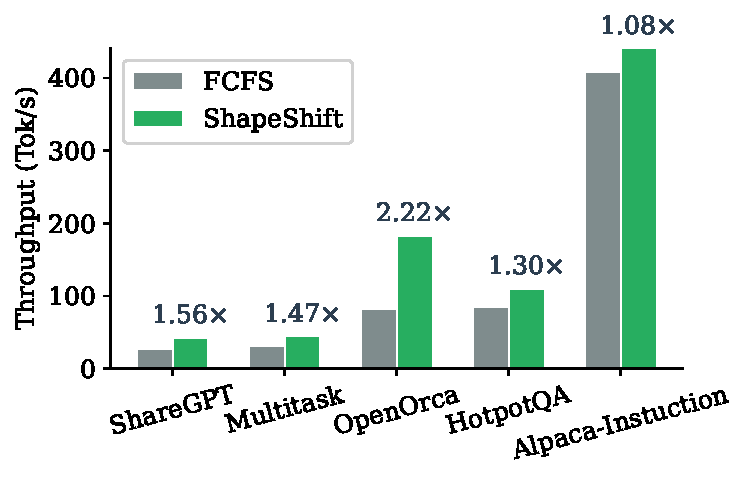
\includegraphics[width=0.30\linewidth]{figures/bar_llada8b_throughput.pdf} &
  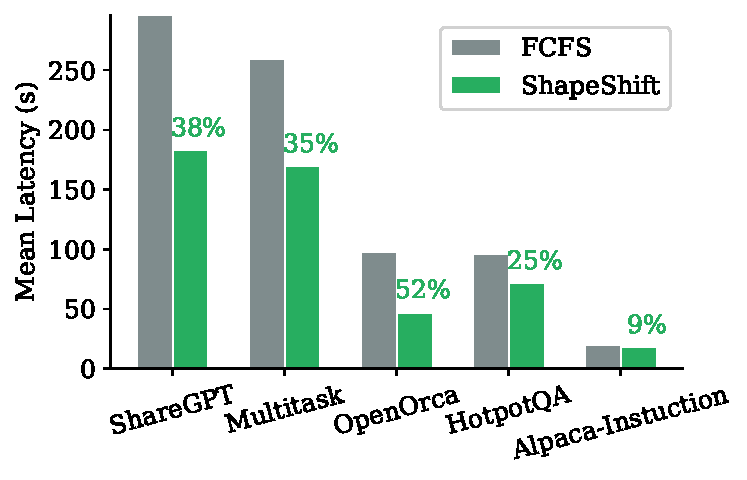
\includegraphics[width=0.30\linewidth]{figures/bar_llada8b_mean.pdf} &
  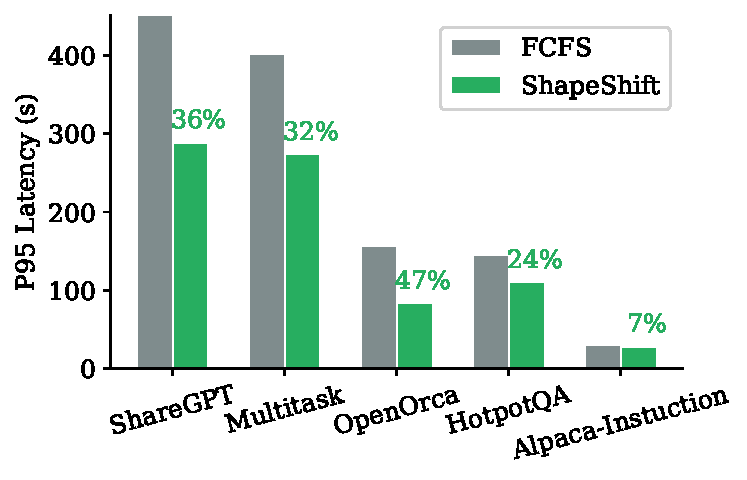
\includegraphics[width=0.30\linewidth]{figures/bar_llada8b_p95.pdf} \\
  \rotatebox{90}{\scriptsize\hspace{6pt}Dream-7B} &
  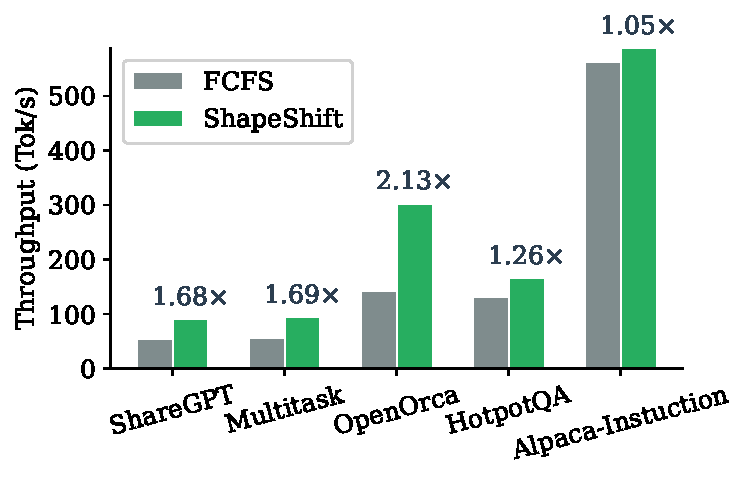
\includegraphics[width=0.30\linewidth]{figures/bar_dream7b_throughput.pdf} &
  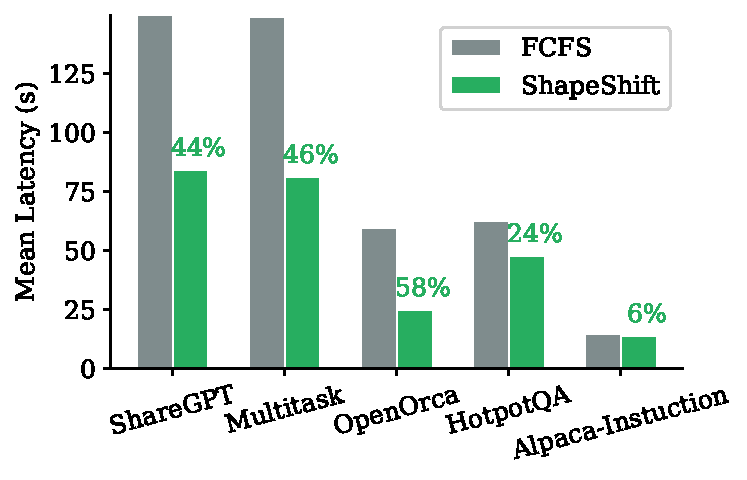
\includegraphics[width=0.30\linewidth]{figures/bar_dream7b_mean.pdf} &
  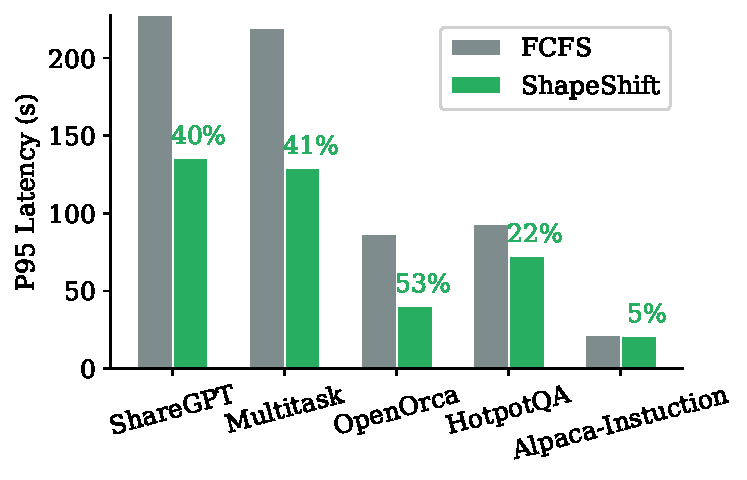
\includegraphics[width=0.30\linewidth]{figures/bar_dream7b_p95.pdf} \\
  \rotatebox{90}{\scriptsize\hspace{6pt}CoDA-1.7B} &
  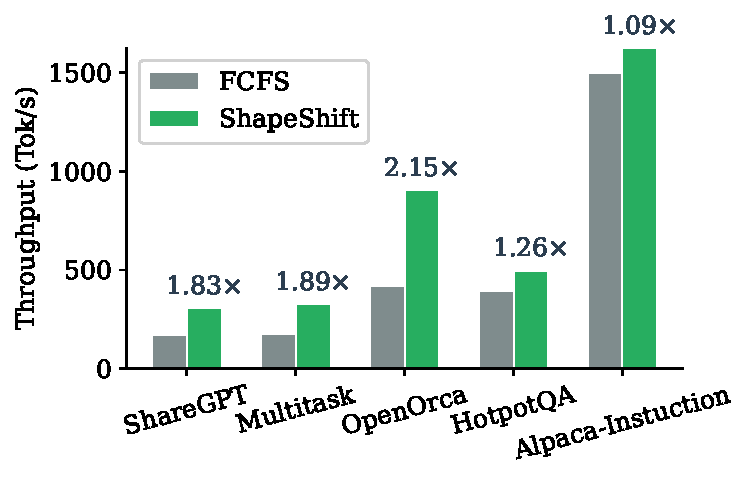
\includegraphics[width=0.30\linewidth]{figures/bar_coda17b_throughput.pdf} &
  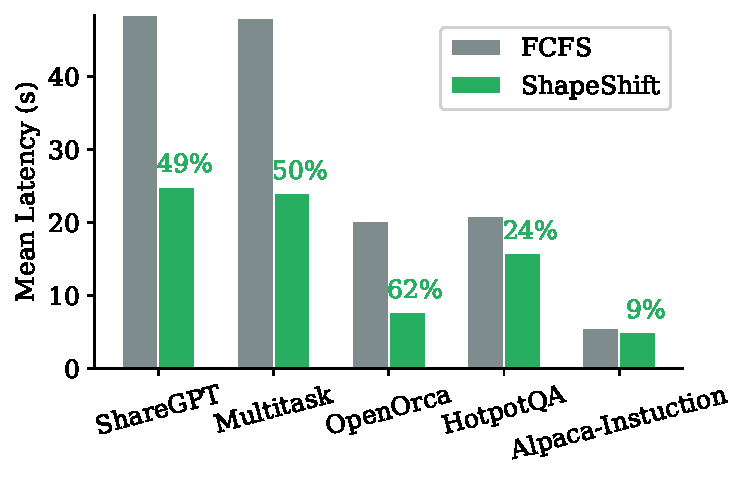
\includegraphics[width=0.30\linewidth]{figures/bar_coda17b_mean.pdf} &
  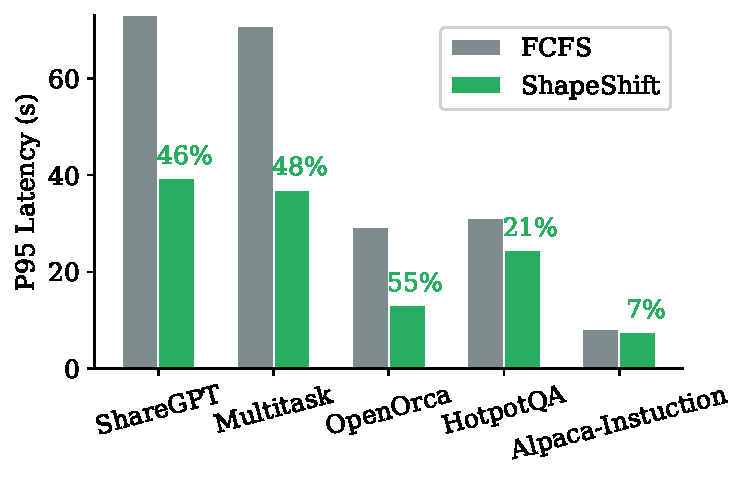
\includegraphics[width=0.30\linewidth]{figures/bar_coda17b_p95.pdf} \\
  \rotatebox{90}{\scriptsize\hspace{6pt}LLaDA2.0-mini} &
  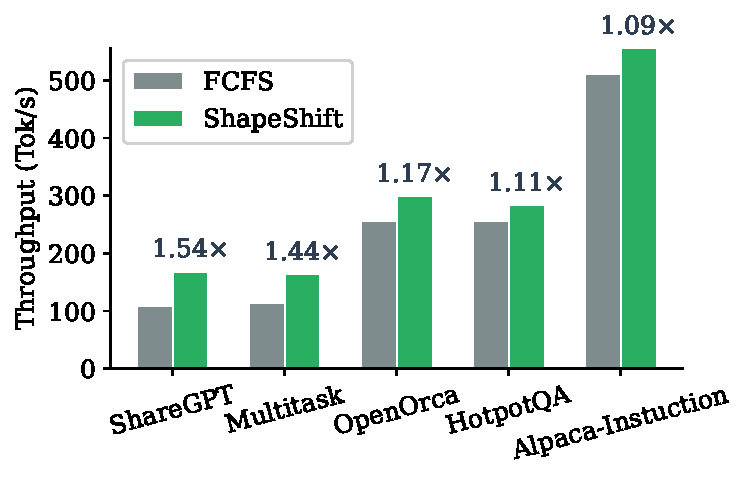
\includegraphics[width=0.30\linewidth]{figures/bar_llada2mini_throughput.pdf} &
  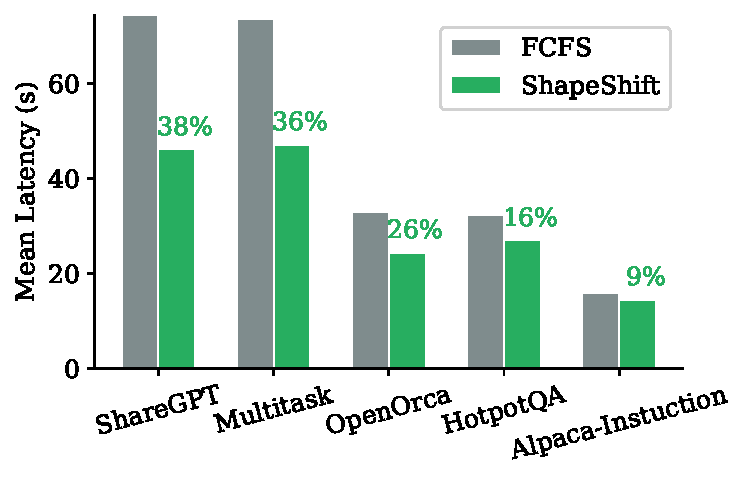
\includegraphics[width=0.30\linewidth]{figures/bar_llada2mini_mean.pdf} &
  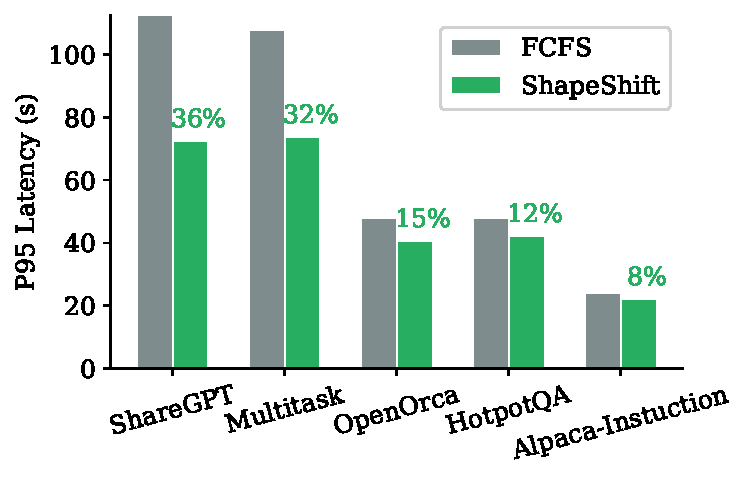
\includegraphics[width=0.30\linewidth]{figures/bar_llada2mini_p95.pdf} \\
  \end{tabular}
  \caption{Online serving results for FCFS and ShapeShift across four checkpoints and five workloads. Rows are checkpoints and columns are metrics. Bar annotations come from a single run; Tables~\ref{tab:main-summary} and~\ref{tab:stronger-baselines} report three-seed means, so LLaDA-8B on OpenOrca reads 2.22$\times$ here and 2.15$\times$ in the tables.}
  \label{fig:main-online}
\end{figure}

Across all checkpoints, ShapeShift improves throughput while also reducing mean and p95 latency relative to FCFS. The throughput gains are consistent across model sizes, indicating that the scheduler is exploiting a serving-level shape effect rather than a checkpoint-specific artifact. Mean latency improves because compact step batches reduce repeated padded transformer work, and p95 latency also drops because service-gap aging keeps shape clustering from turning into long-tail deferral. The improvement is strongest on workloads with long-context spread (up to 2.15$\times$ on OpenOrca), where FCFS repeatedly forms rectangular batches around tail-length requests. LLaDA2.0-mini shows the smallest OpenOrca gain (1.17$\times$), but still improves on every workload.

The latency trends are important for interpreting the throughput gains. ShapeShift is not simply filling the GPU with more work while shifting delay to unlucky requests; throughput improves while both mean and tail latency decrease. This indicates that active-shape batching reduces the amount of work each request repeatedly shares with incompatible companions. The cross-checkpoint pattern also suggests that the opportunity comes from the rectangular serving geometry of dLLM steps, not from a special property of one model implementation.

\subsection{Composition with dInfer}

dInfer~\cite{dInfer2025} and Fast-dLLM~\cite{zhao2025fastdllm} optimize the dLLM generation body, while ShapeShift schedules which requests share repeated denoising batches. Figure~\ref{fig:dinfer-wrapper} tests this separation by placing ShapeShift around a dInfer-backed online wrapper. The wrapper is synchronous and executes one selected batch to completion before selecting the next batch, so the absolute latencies are not directly comparable to dlmserve. The comparison within the wrapper is still meaningful because FCFS and ShapeShift use the same dInfer generation path and differ only in request grouping.

\begin{figure}[t]
\centering
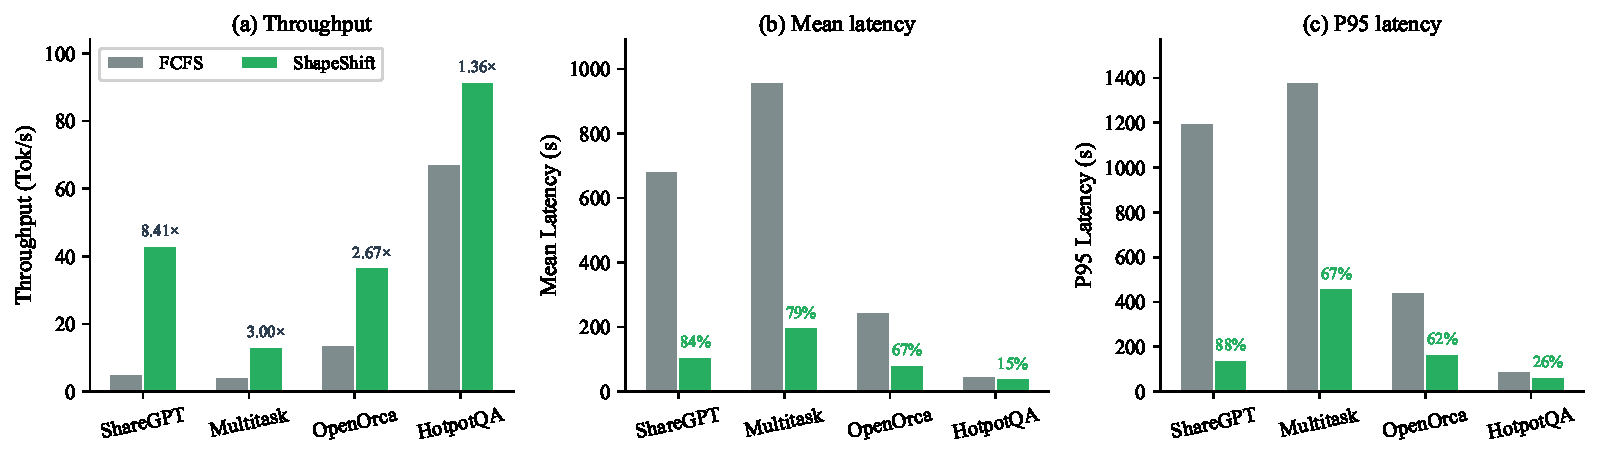
\includegraphics[width=\linewidth]{figures/fig_dinfer_combined.pdf}
\caption{dInfer-backed online wrapper results for FCFS and ShapeShift.}
\label{fig:dinfer-wrapper}
\end{figure}

With the dInfer-backed wrapper, ShapeShift improves online throughput by 1.36--8.41$\times$ across four workloads and reduces p95 latency to 0.12--0.73$\times$ of FCFS under FCFS-matched arrivals. The 8.41$\times$ point is ShareGPT, where FCFS throughput on this synchronous path is 5.12 tok/s and ShapeShift reaches 43.05 tok/s. Multitask and OpenOrca gain 3.00$\times$ and 2.67$\times$. HotpotQA gains 1.36$\times$, the low end of the range, because its prompt lengths are less fragmented. These results show that active-shape scheduling composes with a model-side dLLM acceleration path when both policies share the same generation backend.

\subsection{Mechanism: Shape Waste Drives the Gain}

The mechanism behind the main result is consistent across workloads: higher FCFS step-level padding ratios expose more scheduling headroom. Table~\ref{tab:stress-tests} makes this relationship explicit with synthetic length traces that keep the serving configuration fixed while widening the prompt-length distribution. ``FCFS pad'' and ``Policy pad'' are mean rectangular padding ratios, and the last two columns normalize throughput and p95 latency to FCFS on the same trace. As length heterogeneity increases, FCFS step padding rises from 1.06$\times$ to 2.09$\times$, and ShapeShift throughput gain rises from 1.08$\times$ to 2.31$\times$.

This trend matches the expected boundary behavior. When lengths are similar, FCFS already forms reasonably compact rectangles and the scheduler has little extra shape structure to exploit. As length spread grows, arrival order becomes a worse proxy for compatible co-residence, and FCFS pays more rectangular padding. ShapeShift reduces this padding by selecting companions around a local length region, so both throughput and tail latency improve in the same regime where the measured shape-padding ratio improves.

\subsection{Ablation: Scheduler Components}

Figure~\ref{fig:ablation} separates the design choices on the LLaDA-8B online matrix from Table~\ref{tab:exp-config}. ShapeShift-Shape captures most of the utilization gain from nearest-length active-shape batching. ShapeShift-Aging adds service-gap control on top of that shape-aware batching and improves tail behavior on heterogeneous queues. Full ShapeShift adds compactness filtering; the largest separation appears on OpenOrca, where tighter rectangles recover throughput without sacrificing the aging benefit.

\begin{figure}[t]
\centering
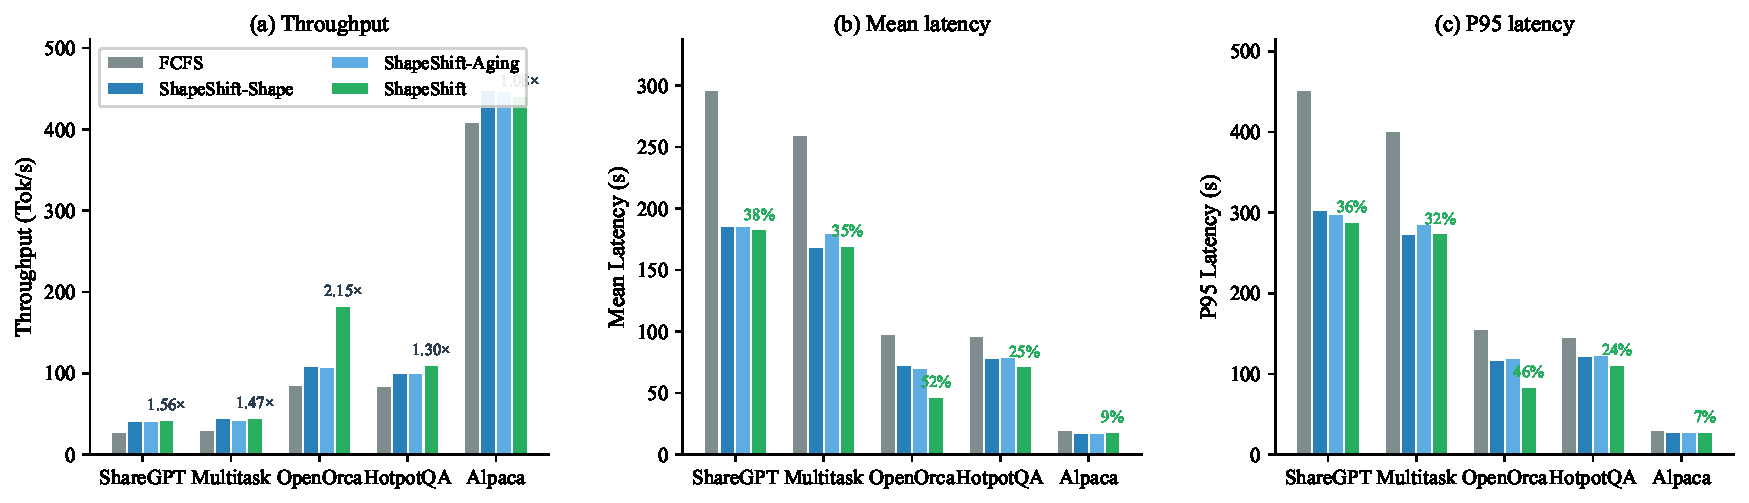
\includegraphics[width=\linewidth]{figures/fig_ablation_combined.pdf}
\caption{Scheduler ablation on LLaDA-8B across five mixed-length serving workloads.}
\label{fig:ablation}
\end{figure}

Table~\ref{tab:stress-tests} also stresses the service-regularity path using a bimodal queue with short, medium, and long outlier requests and a stricter service-gap setting. Shape-only batching reduces padding and improves throughput; aging and the full ShapeShift policy further reduce request latency. In the same service stress, p95 inter-service wait drops from 142.7\,s under FCFS to 62.3\,s with ShapeShift-Shape, 67.3\,s with ShapeShift-Aging, and 57.9\,s with full ShapeShift.

\subsection{Comparison to Stronger Length-Aware Baselines}

Table~\ref{tab:stronger-baselines} compares schedulers that already exploit length information. StaticBucket-FIFO and SJF-Step recover part of the FCFS gap, but SJF-Step keeps p95 near FCFS because aggressive short-first packing defers long requests. Full ShapeShift is the only policy that simultaneously improves throughput and tail latency on the most heterogeneous queue (OpenOrca: 2.15$\times$ throughput at 0.54 normalized p95, vs.\ 1.66$\times$ at 0.88 for the best stronger baseline).

\begin{table}[t]
\centering
\caption{Stronger scheduler baselines on the LLaDA-8B matrix. Each cell reports throughput speedup over FCFS and p95 latency normalized to FCFS.}
\label{tab:stronger-baselines}
\scriptsize
\setlength{\tabcolsep}{3.0pt}
\resizebox{\columnwidth}{!}{%
\begin{tabular}{lcccc}
\toprule
Workload & StaticBucket-FIFO & SJF-Step & LengthBucket & ShapeShift \\
\midrule
ShareGPT & 1.37$\times$ / 0.77 & 1.54$\times$ / 0.95 & 1.50$\times$ / 0.67 & 1.56$\times$ / 0.64 \\
Multitask & 1.30$\times$ / 0.79 & 1.41$\times$ / 1.03 & 1.47$\times$ / 0.68 & 1.47$\times$ / 0.68 \\
OpenOrca & 1.51$\times$ / 0.75 & 1.66$\times$ / 0.88 & 1.28$\times$ / 0.75 & 2.15$\times$ / 0.54 \\
HotpotQA & 1.14$\times$ / 0.85 & 1.19$\times$ / 1.02 & 1.19$\times$ / 0.84 & 1.30$\times$ / 0.76 \\
Alpaca & 1.05$\times$ / 0.94 & 1.07$\times$ / 0.99 & 1.10$\times$ / 0.91 & 1.08$\times$ / 0.93 \\
\midrule
Geo. mean & 1.26$\times$ / 0.82 & 1.35$\times$ / 0.97 & 1.30$\times$ / 0.76 & 1.47$\times$ / 0.70 \\
\bottomrule
\end{tabular}
}
\end{table}

\begin{table}[t]
\centering
\caption{Shape-heterogeneity and service-regularity stress tests in dlmserve.}
\label{tab:stress-tests}
\scriptsize
\setlength{\tabcolsep}{2.5pt}
\resizebox{\columnwidth}{!}{%
\begin{tabular}{llrrrr}
\toprule
Stress & Setting / Policy & FCFS pad & Policy pad & Tput/FCFS & P95/FCFS \\
\midrule
Heterogeneity & Low-CV trace & 1.06 & 1.03 & 1.08$\times$ & 0.93 \\
Heterogeneity & Medium-CV trace & 1.57 & 1.11 & 1.91$\times$ & 0.52 \\
Heterogeneity & High-CV trace & 2.09 & 1.21 & 2.31$\times$ & 0.43 \\
\midrule
Service & ShapeShift-Shape & 2.39 & 1.62 & 1.71$\times$ & 0.58 \\
Service & ShapeShift-Aging & 2.39 & 1.37 & 2.13$\times$ & 0.47 \\
Service & ShapeShift & 2.39 & 1.37 & 2.14$\times$ & 0.47 \\
\bottomrule
\end{tabular}
}
\end{table}

Figure~\ref{fig:fullstep} validates the longer online path on five workloads: ShapeShift-Shape improves throughput by 1.14--1.88$\times$ and reduces p95 latency to 0.53--0.88$\times$ of FCFS; ShapeShift-Aging adds an explicit service-gap knob while preserving most of the gain.

\begin{figure}[t]
\centering
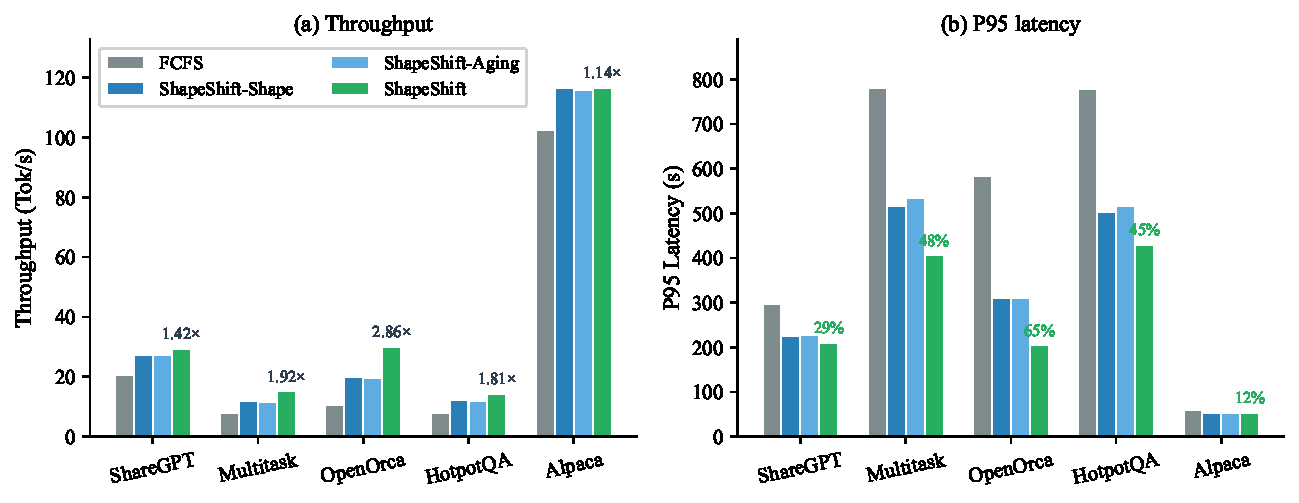
\includegraphics[width=\linewidth]{figures/fig_fullstep_combined.pdf}
\caption{Longer-horizon online validation across five serving workloads on LLaDA-8B.}
\label{fig:fullstep}
\end{figure}

\subsection{Burst Replay and Operating Boundaries}

Production serving also sees bursty session structure. Table~\ref{tab:burst-replay} replays sessionized ShareGPT and Multitask arrivals while scaling inter-arrival gaps.

\begin{table}[t]
\centering
\caption{Burst-replay validation. Each cell reports throughput speedup over FCFS and p95 latency normalized to FCFS.}
\label{tab:burst-replay}
\scriptsize
\setlength{\tabcolsep}{3.2pt}
\resizebox{\columnwidth}{!}{%
\begin{tabular}{llccc}
\toprule
Trace & Replay scale & ShapeShift-Shape & ShapeShift-Aging & ShapeShift \\
\midrule
ShareGPT & 1.5$\times$ spacing & 1.04$\times$ / 0.95 & 1.03$\times$ / 0.96 & 1.05$\times$ / 0.92 \\
ShareGPT & 1.0$\times$ spacing & 1.18$\times$ / 0.83 & 1.15$\times$ / 0.85 & 1.20$\times$ / 0.78 \\
ShareGPT & 0.75$\times$ spacing & 1.30$\times$ / 0.74 & 1.27$\times$ / 0.77 & 1.33$\times$ / 0.71 \\
Multitask & 1.5$\times$ spacing & 1.06$\times$ / 0.94 & 1.04$\times$ / 0.95 & 1.07$\times$ / 0.90 \\
Multitask & 1.0$\times$ spacing & 1.26$\times$ / 0.79 & 1.22$\times$ / 0.82 & 1.32$\times$ / 0.69 \\
Multitask & 0.75$\times$ spacing & 1.49$\times$ / 0.67 & 1.41$\times$ / 0.71 & 1.56$\times$ / 0.58 \\
\bottomrule
\end{tabular}
}
\end{table}

Under light replay ($1.5\times$ spacing) the policies converge toward FCFS; at $0.75\times$ spacing the gap reopens, up to 1.56$\times$ throughput at 0.58 normalized p95 on Multitask. 

Backlog determines whether active-shape scheduling has companions to choose from. On the all-ready ShareGPT multi-turn trace, ShapeShift-Shape and ShapeShift-Aging improve throughput by 1.37$\times$ and 1.30$\times$ while reducing p95 latency to 0.73$\times$ and 0.77$\times$ of FCFS. With 100--500\,ms arrival spreading, the ready pool becomes thin and both policies converge to FCFS, with throughput at 0.99--1.02$\times$ and p95 at 0.98--1.04$\times$. Length dispersion shows the same boundary from the padding side: Table~\ref{tab:stress-tests} links higher FCFS padding ratios to larger ShapeShift gains. Together, these results define the intended operating regime---backlogged, shape-heterogeneous online queues---rather than a claim of universal speedup.

\section{Related Work}

\textbf{LLM serving systems.} Orca~\cite{orca2022}, vLLM~\cite{vllm2023}, DistServe~\cite{distserve2024}, and Sarathi-Serve~\cite{sarathi2024} shape modern LLM-serving evaluation through matched baselines, load sweeps, and throughput under latency constraints. Beyond these canonical baselines, recent serving work studies phase splitting, speculative verification, multi-tenant adapter batching, multi-model multiplexing, and cross-request KV-cache reuse across memory tiers~\cite{splitwise2023,specinfer2024,medusa2024,eagle2024,tetriinfer2024,punica2023,slora2023,muxserve2024,mcam2025}. Memory for model adaptation, such as compositional concept-graph memory for vision--language models~\cite{zhou2026comem}, sits outside this serving-time KV residency. Their scheduling problem is organized around AR prefill/decode, KV-cache residency, and incremental token generation. ShapeShift adopts this evaluation methodology, but targets a dLLM cost where length becomes a recurring step-batch resource rather than a prefill attribute.

\textbf{dLLM inference and serving.} Recent dLLM execution work improves cache reuse, sparse attention, or focused computation~\cite{zhao2025fastdllm,dllmcache2025,d2cache2025,dkvcache2025,sparsedllm2025,focuscompute2026,focusdllm2026}. Serving-oriented systems such as dInfer, dLLM-Serve, vLLM-Omni, and dlmserve address iteration management and online deployment~\cite{dInfer2025,dllmserve2025,vllmomni2026,dlmserve2026}. These systems reduce the cost of executing a chosen update or managing the update loop. ShapeShift instead changes the active-set decision that creates the update shape.

\textbf{Diffusion and long-context serving.} DiT-Serve~\cite{ditserve2025}, GenServe~\cite{genserve2026}, and DisagFusion~\cite{disagfusion2026} treat diffusion updates as a serving schedule for image and video workloads, and interactive 3D scene generation~\cite{li2026comprehensive} adds user-in-the-loop generative workloads with their own iterative refinement. ShapeShift applies this perspective to text dLLMs, where the repeated shape resource is variable sequence-length padding in a bidirectional token transformer. AR long-context systems such as LoongServe~\cite{loongserve2024}, AlignedServe~\cite{alignedserve2026}, and LAPS~\cite{laps2026} also motivate length-aware scheduling, but AR decoding amortizes the prompt through KV-cache reuse and then advances one token at a time. Multimodal pipelines such as composed image and video retrieval~\cite{encoder2025,offset2025,hud2025,pair2025}, which pair a reference visual with a modification text, further diversify what each request carries; these works improve retrieval quality and leave step-level batching open.

\textbf{Variable-length generation and per-request cost.} Earlier text diffusion models such as SSD-LM~\cite{ssdlm2022}, DiffuLLaMA~\cite{diffullama2024}, and iLLaDA~\cite{illada2026} expand the non-autoregressive text-generation family toward stronger open dLLMs, and length-aware dLLM methods~\cite{nativelength2026} reduce wasted output canvas. Orthogonal work lowers per-request cost before a request reaches the scheduler: frequency-aligned and task-aware memory distillation~\cite{li2025frequency,li2026tam} yield lightweight predictors, dataset distillation~\cite{li2025ddtime} shrinks the data a model is trained on, layer-wise information allocation~\cite{li2026rethinking} and federated soft-prompt adaptation~\cite{xiao2026prototype} change how a foundation model is adapted or conditioned, and work on reasoning-trace pruning~\cite{jiang2025drp}, teacher distillation~\cite{zhang2025find}, memorization-constrained reasoning~\cite{jiang2026beyond}, and tool-use supervision~\cite{xu2025learning,jiang2026scribe} shapes how long and how structured model outputs are. These methods change the length $L_r$ or per-token cost of individual requests, and thereby the length distribution a server sees; active-shape scheduling reduces padding between the heterogeneous requests that remain in the same online batch.

\section{Limitations and Scope}

ShapeShift targets online text dLLM queues where the ready pool is both backlogged and length-heterogeneous. Under thin offered load or narrow prompt-length distributions, the ready pool contains fewer shape-compatible companions and the gain naturally approaches FCFS, as shown by the spread-arrival and light burst-replay settings.

This paper isolates the single-GPU step-batch decision. We do not study multi-GPU tensor parallelism, request migration, or cluster-level admission control. A production deployment would also need to co-tune compactness and service-gap budgets with SLA targets; our evaluation uses the dlmserve defaults shared across all online runs. The dInfer composition experiment uses a synchronous wrapper and should be read as a same-path scheduler comparison rather than an absolute latency benchmark against dlmserve. Finally, ShapeShift changes only which requests share a step; output-quality interventions such as character-level error correction~\cite{lin2026cec} are outside its scope.

\section{Conclusion}

Long-context dLLM serving introduces a repeated shape-padding problem: short requests batched with long requests pay the long request's transformer shape across repeated denoising updates. ShapeShift treats sequence shape as a step-level scheduling resource, using active-shape batching, compactness filtering, and service-gap aging to recover utilization while preserving service regularity. On dlmserve, ShapeShift improves throughput by 1.11--2.15$\times$ over FCFS across four checkpoints and mixed-length traces, while reducing mean and p95 latency. Longer-horizon validation shows 1.14--1.88$\times$ gains across five workloads. The results support a simple principle for dLLM serving systems: schedule not only when requests run, but also which sequence shapes run together.

\begin{credits}
\subsubsection*{Disclosure of Interests}
The authors have no competing interests to declare that are relevant to the content of this article.
\end{credits}

\bibliographystyle{splncs04}
\bibliography{references}

\end{document}
